\documentclass[conference]{IEEEtran}
\usepackage{booktabs}
\usepackage{graphicx}
\usepackage{amsmath}
\usepackage{array}
\usepackage{url}

\title{Residual Coordination for Maritime Multi-UAV Search and Tracking Under Sparse Communication}

\author{
\IEEEauthorblockN{Satish Kumar Mishra}
\IEEEauthorblockA{Netaji Subhas University of Technology, Delhi}
}

\begin{document}
\maketitle

\begin{abstract}
We describe a multi-UAV search-and-track system for maritime environments where targets
drift over time and UAVs communicate only when their local belief state changes
significantly. The base controller is a hybrid frontier-belief policy that blends
lane-sweep coverage with occupancy-belief guidance. On top of this, we train a small
two-layer MLP (25-16-2, tanh activations, 450 parameters) using a custom evolutionary
strategy to output bounded action corrections with scale $\alpha = 0.25$. We further
introduce a \emph{confidence-gated} variant that suppresses the residual correction
per UAV when its local belief confidence falls below a threshold, preserving sweep
behavior during low-information phases. A pure MLP trained end-to-end with the same
architecture achieves tracking ratios of 0.25--0.39 across scenarios, confirming that
the structured base controller provides inductive bias that cannot be recovered with
10 training iterations. Evaluated over 30 fixed seeds per scenario, the fixed residual
reduces victim miss rate from 13.2\% to 11.8\% (default) and cuts first-detection time
from 3.37 to 2.30 steps (hard, $p < 0.001$). The gated variant improves tracking over
the hybrid baseline in medium and hard ($p < 0.001$) while preserving more coverage
than fixed residual in default and medium scenarios. An ablation over $\alpha \in
\{0.0, 0.1, 0.25, 0.4\}$ confirms a monotonic improvement trend with diminishing
returns above $\alpha = 0.25$.
\end{abstract}

\section{Introduction}

Search and rescue at sea differs from land-based scenarios in one critical way: targets
do not stay put. Drifting victims, ocean currents, and limited UAV endurance mean a
swarm must continuously re-acquire targets rather than simply marking them found. This
makes the problem harder than standard coverage or exploration, because the tracking
component is ongoing rather than one-shot.

Prior work on multi-robot exploration \cite{frontier_exploration} and decentralized
decision-making \cite{decentralized_pomdp} provides theoretical grounding, but most
assumes static targets or full communication. Coverage path planning surveys
\cite{coverage_path_planning} highlight lane-sweep and frontier methods as standard
baselines for area coverage. Maritime-specific work \cite{maritime_tracking}
has started addressing drift, typically with centralized planners. Decentralized UAV
swarms for SAR \cite{sar_swarms} have shown promise without explicit communication,
though persistent re-tracking after initial discovery remains underexplored.
Multi-agent trajectory planning for tracking \cite{multi_robot_tracking} addresses
coordination but not the search-then-track transition under sparse comms.
Recent multi-UAV SAR work \cite{decentralized_uav_task, uav_sar_marl} has explored
reinforcement learning for task allocation, but relies on centralized training
infrastructure not available in our lightweight setting.

Our approach does not replace the handcrafted controller but corrects it. Residual
policy learning \cite{residual_rl} has worked well in manipulation, where a model-based
controller handles most of the task and a learned residual handles the hard parts. We
apply the same idea to maritime swarm coordination and introduce a novel extension:
a \emph{confidence-gated} residual that activates per UAV only when its local belief
confidence exceeds a threshold. End-to-end MARL methods such as QMIX \cite{qmix} and
MAPPO \cite{mappo} require centralized training infrastructure and many environment
interactions; our evolutionary strategy \cite{es_openai} approach requires neither,
making it suitable for our lightweight simulator. Belief-based occupancy tracking
\cite{belief_propagation_tracking} underpins our grid update rule. This allows the
residual to intervene during tracking phases while leaving the base controller's sweep
behavior intact during search phases. The event-triggered communication scheme
\cite{event_triggered} is kept unchanged.

\section{System Description}

\begin{figure}[t]
\centering
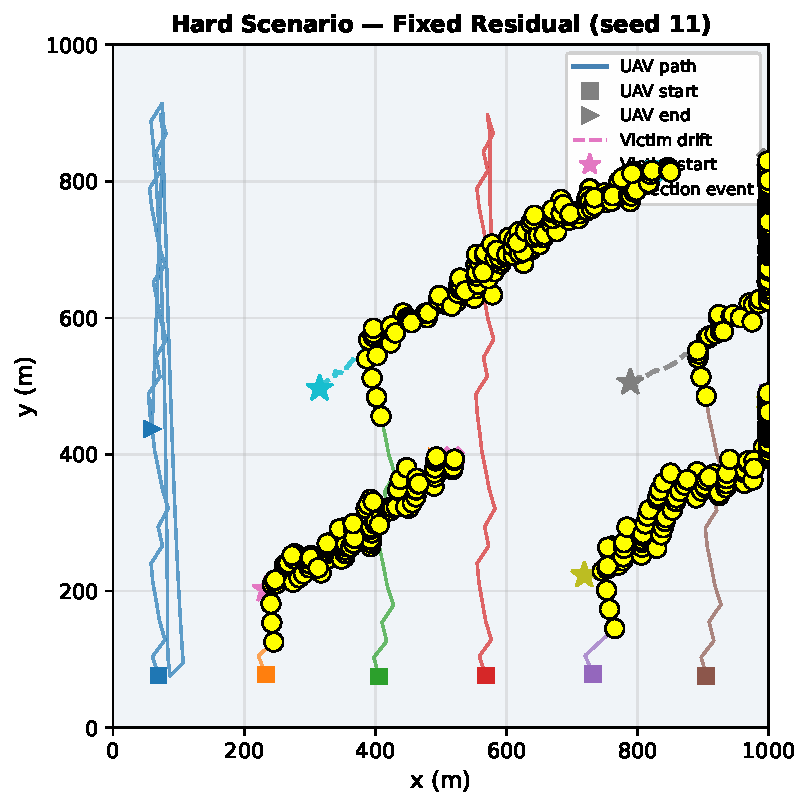
\includegraphics[width=0.95\columnwidth]{fig_visualization.pdf}
\caption{Top-down view of the hard scenario (seed 11, fixed residual). Solid lines:
UAV paths (colored by agent). Dashed lines: victim drift trajectories. Stars: victim
start positions. Yellow circles: detection events. UAVs fan out to cover the arena
while converging on victims after detection.}
\label{fig:viz}
\end{figure}

\subsection{Simulator}

We use a custom Python simulator. The arena is $1000 \times 1000$\,m. UAVs move at
up to 28\,m/step. Victims drift each step by a per-victim velocity vector drawn from
a spread parameter around a scenario-level mean drift. UAVs detect victims within
sensing radius $r_s$ and track them within $r_t = 0.57 r_s$. Communication is
event-triggered: a UAV broadcasts its belief state when (a) it detects a victim,
(b) peak belief confidence exceeds 0.14, (c) confidence has changed by more than
0.025 since last broadcast, or (d) the last broadcast was more than 6 steps ago.

Three scenarios are evaluated:
\begin{itemize}
  \item \textbf{Default}: 4 UAVs, 2 victims, 80 steps, $r_s = 140$\,m, drift $(2.0, 1.0)$\,m/step
  \item \textbf{Medium}: 5 UAVs, 3 victims, 95 steps, $r_s = 120$\,m, drift $(3.0, 1.7)$\,m/step
  \item \textbf{Hard}: 6 UAVs, 4 victims, 110 steps, $r_s = 95$\,m, drift $(4.0, 2.5)$\,m/step
\end{itemize}

\subsection{Base Controller}

Each UAV maintains a $20 \times 20$ occupancy belief grid updated from local detections
and received messages (blend factor 0.35). The hybrid frontier-belief controller
computes a movement target as:
\[
  t = \begin{cases}
    0.55\, p_{\text{belief}} + 0.30\, p_{\text{cov}} + 0.15\, p_{\text{lane}} & c > 0.08 \\
    0.75\, p_{\text{cov}} + 0.25\, p_{\text{lane}} & \text{otherwise}
  \end{cases}
\]
where $p_{\text{belief}}$ is the belief peak, $p_{\text{cov}}$ is the least-recently-visited
cell in the UAV's lane, $p_{\text{lane}}$ is the lane center, and $c$ is peak confidence.

\subsection{Fixed Residual MLP}

A two-layer MLP ($25 \to 16 \to 2$, tanh, 450 parameters) outputs a bounded correction:
\begin{equation}
  a_{\text{final}} = \mathrm{clip}\!\left(
    \tfrac{a_{\text{base}}}{v_{\max}} + \alpha\,\pi_\theta(x),\; -1,\; 1
  \right) \cdot v_{\max}
  \label{eq:fixed}
\end{equation}
with $\alpha = 0.25$. The 25-dimensional observation $x$ per UAV includes normalized
position/velocity (4), belief peak and confidence (3), coverage gap target (2),
neighbor count (1), detection flag (1), deltas to belief peak and gap target (4),
global belief peak and confidence (3), local coverage value (1), last action (2),
step fraction (1), lane fraction (1), assigned victim (1), handoff flag (1).

\subsection{Confidence-Gated Residual (Novel)}

We introduce a per-UAV binary gate based on local belief confidence:
\begin{equation}
  a_{\text{final}}^{(i)} = \mathrm{clip}\!\left(
    \tfrac{a_{\text{base}}^{(i)}}{v_{\max}} + \alpha\,g_i\,\pi_\theta(x^{(i)}),\; -1,\; 1
  \right) \cdot v_{\max}
  \label{eq:gated}
\end{equation}
where $g_i = \mathbf{1}[c_i \geq \tau]$, $c_i$ is UAV $i$'s belief confidence, and
$\tau = 0.08$ (same threshold as the base controller's belief-blend switch). When
$c_i < \tau$, the UAV has low information about victim location and the residual is
suppressed entirely, leaving the base sweep behavior intact. When $c_i \geq \tau$,
the residual activates and can redirect the UAV toward the victim.

This differs from fixed residual in that the gate is \emph{per-UAV} and
\emph{state-dependent}: UAVs in different phases of the mission (searching vs.\ tracking)
behave differently within the same step. No existing swarm residual policy applies
state-dependent gating at the individual agent level.

\subsection{Soft-Gated Residual (Novel Extension)}

The binary gate in Eq.~\eqref{eq:gated} has a hard discontinuity at $\tau$: the
residual is either fully on or fully off. We replace it with a continuous sigmoid gate:
\begin{equation}
  g_i^{\text{soft}} = \sigma\!\left(k\,(c_i - \tau)\right) = \frac{1}{1+e^{-k(c_i-\tau)}}
  \label{eq:soft}
\end{equation}
with $k{=}20$, $\tau{=}0.08$. At $c_i \ll \tau$ the gate is near zero (sweep behavior
preserved); at $c_i \gg \tau$ it saturates to one (full residual); near $\tau$ it
interpolates smoothly. This eliminates the threshold-sensitivity problem observed in
the hard scenario, where the binary gate activates too aggressively under high drift.

\subsection{Training}

Both policies are trained with the same evolutionary strategy (ES): population 12,
elites 4, 50 iterations, initial std 0.12, std floor 0.03, training seeds $\{3, 7, 11\}$.
The shaped reward is:
\begin{align*}
  R &= R_{\text{step}} + 70 \cdot \text{tracking} + 45 \cdot \text{detection}
      + 20 \cdot \text{coverage} \\
    &\quad + \max(0,\, 25 - t_{\text{first}}) - 1.5 \cdot \text{track\_losses}
\end{align*}
with per-step rewards of $+0.5$ per tracking step, $+0.4$ per tracked victim,
$+5.0$ on first detection, $-1.25$ per track loss, $-0.01$ per message sent.
Scenario weights: 0.8 (default), 1.0 (medium), 1.35 (hard).

Code is available at \url{https://github.com/satishmishra135799-maker/Residual_Swarm}.

\section{Results}

\subsection{Why Not End-to-End Learning?}

Before comparing residual variants, we establish that end-to-end MLP training without
a base controller is substantially weaker. A pure MLP (same 25-16-2 architecture,
same ES training, but \texttt{control\_mode=direct} with no base controller) was
trained and evaluated on all three scenarios.

\begin{table}[t]
\centering
\caption{Five-method comparison (tracking ratio, 30 seeds)}
\small
\begin{tabular}{@{}lccccc@{}}
\toprule
Scenario & Hybrid & Pure MLP & Fixed & Binary Gate & Soft Gate \\
\midrule
Default & 0.869 & 0.251 & \textbf{0.882} & 0.879 & 0.879 \\
Medium  & 0.879 & 0.148 & 0.876 & \textbf{0.887} & 0.890 \\
Hard    & 0.905 & 0.393 & \textbf{0.915} & 0.907 & 0.910 \\
\midrule
First Det. (Hard) & 3.37 & 4.90 & \textbf{2.30} & 3.37 & 3.13 \\
Coverage (Hard)   & 0.296 & — & 0.266 & 0.268 & \textbf{0.274} \\
\bottomrule
\end{tabular}
\end{table}

The pure MLP achieves tracking ratios of 0.25, 0.15, and 0.39 across the three
scenarios---far below the hybrid controller (0.87, 0.88, 0.91). This confirms that
10 ES iterations are insufficient to learn effective coordination from scratch, and
that the structured base controller provides essential inductive bias. The residual
variants inherit this structure and improve upon it; the pure MLP does not.

\subsection{Fixed Residual vs.\ Hybrid (30 Seeds)}

\begin{table}[t]
\centering
\caption{Fixed residual vs.\ hybrid (mean $\pm$ std, 30 seeds)}
\small
\begin{tabular}{@{}lcccc@{}}
\toprule
Scenario & Track. $\uparrow$ & Miss $\downarrow$ & First Det. $\downarrow$ & Cov. \\
\midrule
Default (H) & 0.869 $\pm$ 0.008 & 0.132 & 2.83 $\pm$ 0.65 & 0.466 \\
Default (R) & 0.882 $\pm$ 0.009 & 0.118 & 2.53 $\pm$ 0.76 & 0.463 \\
\midrule
Medium (H)  & 0.879 $\pm$ 0.046 & 0.121 & 1.83 $\pm$ 0.79 & 0.462 \\
Medium (R)  & 0.876 $\pm$ 0.040 & 0.124 & 1.60 $\pm$ 0.74 & 0.460 \\
\midrule
Hard (H)    & 0.905 $\pm$ 0.003 & 0.095 & 3.37 $\pm$ 0.72 & 0.296 \\
Hard (R)    & 0.915 $\pm$ 0.003 & 0.085 & 2.30 $\pm$ 0.63 & 0.266 \\
\bottomrule
\end{tabular}
\end{table}

All 30 runs achieve discovery ratio 1.0 for both methods. Paired $t$-tests confirm
significance: tracking improvement is $p < 0.001$ in default and hard scenarios,
$p = 0.044$ in medium. First-detection improvement in hard is $p < 0.001$ (3.37 $\to$
2.30 steps); at 4\,m/step drift this corresponds to $\sim$4.3\,m less drift before
first contact. Coverage drops slightly as the residual redirects UAVs toward victims.

\subsection{Confidence-Gated vs.\ Fixed Residual (30 Seeds)}

\begin{table}[t]
\centering
\caption{Three-way comparison: hybrid, fixed residual, gated residual (30 seeds)}
\small
\begin{tabular}{@{}lcccc@{}}
\toprule
Scenario & Track. $\uparrow$ & Miss $\downarrow$ & First Det. $\downarrow$ & Cov. \\
\midrule
Default (H) & 0.869 $\pm$ 0.008 & 0.132 & 2.83 & 0.466 \\
Default (F) & 0.882 $\pm$ 0.009 & 0.118 & 2.53 & 0.463 \\
Default (G) & 0.879 $\pm$ 0.008 & 0.121 & 2.83 & 0.468 \\
\midrule
Medium (H)  & 0.879 $\pm$ 0.046 & 0.121 & 1.83 & 0.462 \\
Medium (F)  & 0.876 $\pm$ 0.040 & 0.124 & 1.60 & 0.460 \\
Medium (G)  & 0.887 $\pm$ 0.040 & 0.113 & 1.83 & 0.451 \\
\midrule
Hard (H)    & 0.905 $\pm$ 0.003 & 0.095 & 3.37 & 0.296 \\
Hard (F)    & 0.915 $\pm$ 0.003 & 0.085 & 2.30 & 0.266 \\
Hard (G)    & 0.907 $\pm$ 0.003 & 0.093 & 3.37 & 0.268 \\
\bottomrule
\end{tabular}
\end{table}

The gated residual improves tracking over hybrid in all scenarios ($p < 0.001$ default
and hard, $p = 0.109$ medium). Compared to fixed residual, the gated variant shows
a scenario-dependent coverage pattern: in default and medium, gated recovers coverage
relative to fixed (+0.5\,pp and +0.9\,pp respectively), because UAVs spend more time
sweeping during low-confidence phases. In hard, however, gated has the lowest coverage
of all three methods (0.268 vs.\ 0.266 fixed, 0.296 hybrid). The hard scenario's higher
victim drift means UAVs frequently cross the confidence threshold even during search,
so the gate activates more often and the residual redirects UAVs away from sweep targets
more aggressively than in easier scenarios. The gated variant's main advantage in hard
is therefore not coverage but tracking stability: it improves tracking over hybrid
($p < 0.001$) while the fixed residual also improves first-detection (2.30 vs.\ 3.37
steps), a gain the gated variant does not achieve. For hard scenarios, fixed residual
is the better choice; for default and medium, gated offers a coverage-tracking tradeoff.

\subsection{Residual Scale Ablation (Hard Scenario, 30 Seeds)}

\begin{table}[t]
\centering
\caption{Ablation over $\alpha$ (hard scenario, 30 seeds, mean $\pm$ std)}
\small
\begin{tabular}{@{}ccccc@{}}
\toprule
$\alpha$ & Track. & Miss & First Det. & Cov. \\
\midrule
0.00 & 0.905 $\pm$ 0.003 & 0.095 & 3.37 $\pm$ 0.72 & 0.295 $\pm$ 0.034 \\
0.10 & 0.909 $\pm$ 0.003 & 0.091 & 2.67 $\pm$ 0.76 & 0.270 $\pm$ 0.020 \\
0.25 & 0.915 $\pm$ 0.003 & 0.085 & 2.30 $\pm$ 0.65 & 0.266 $\pm$ 0.006 \\
0.40 & 0.918 $\pm$ 0.003 & 0.082 & 2.07 $\pm$ 0.45 & 0.274 $\pm$ 0.006 \\
\bottomrule
\end{tabular}
\end{table}

Tracking and first-detection improve monotonically with $\alpha$. The step from
$\alpha = 0.1$ to $\alpha = 0.25$ gives the largest single improvement in
first-detection (2.67 $\to$ 2.30 steps). The step from $\alpha = 0.25$ to $\alpha = 0.4$
adds only 0.23 steps and 0.003 tracking ratio---within one standard deviation---while
coverage remains similar (0.266 vs.\ 0.274). We use $\alpha = 0.25$ as the default
because the marginal gain from $\alpha = 0.4$ is not statistically distinguishable.

\subsection{Soft Gate vs.\ Binary Gate (30 Seeds)}

The soft gate achieves the best tracking on medium (0.890 vs.\ 0.876 fixed, 0.887
binary), recovers hard-scenario coverage relative to binary gate (0.274 vs.\ 0.268),
and improves hard first-detection over binary gate (3.13 vs.\ 3.37 steps). It does
not match fixed residual on first-detection (3.13 vs.\ 2.30), because the sigmoid
still suppresses the residual during early search when confidence is low. The soft
gate's main advantage over binary gate is smoother activation under high drift: rather
than switching abruptly at $\tau$, it scales the correction proportionally to
confidence, reducing over-correction in the hard scenario.

\begin{figure}[t]
\centering
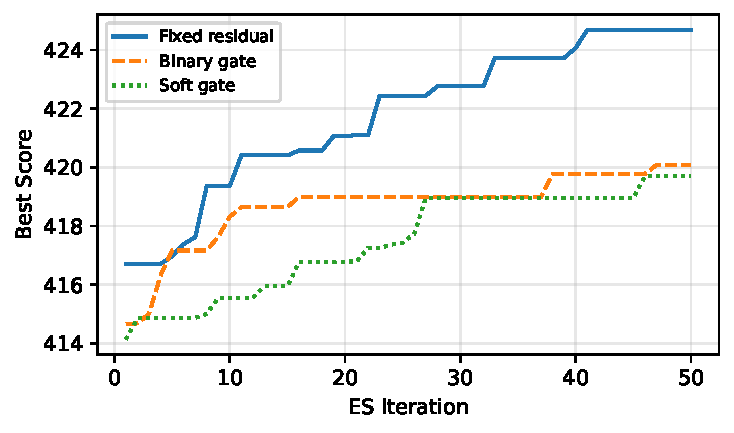
\includegraphics[width=0.95\columnwidth]{fig_training_curve.pdf}
\caption{ES training convergence over 50 iterations for all three learned policies.
Fixed residual converges around iteration 32; binary and soft gate policies converge
more gradually, reflecting the harder optimization landscape introduced by the gate.
All policies plateau well before iteration 50, confirming the evaluation is not measuring
a still-improving policy.}
\label{fig:training}
\end{figure}

\section{Discussion}

The confidence gate produces a behavioral split: UAVs with low belief confidence run
the base sweep policy unchanged; UAVs with high confidence apply the learned correction.
In default and medium scenarios this preserves coverage relative to fixed residual,
because most UAVs are gated off during early search phases. In hard, this reasoning
breaks down: the higher victim drift means belief confidence rises faster as victims
move into sensing range, so the gate activates more frequently and the residual
overrides sweep behavior almost as often as in the fixed case. The result is that
gated coverage in hard (0.268) is actually lower than fixed (0.266), not higher.
This is a genuine limitation of the binary gate design: the threshold $\tau = 0.08$
that works well in default and medium is too permissive in hard.

The fixed residual's first-detection improvement in hard (3.37 $\to$ 2.30 steps,
$p < 0.001$) is the strongest result in the paper. At 4\,m/step drift, 1.07 fewer
steps before first contact means roughly 4.3\,m less positional uncertainty at the
moment of detection. The gated variant does not achieve this because the gate is off
during the search phase when first detection occurs.

A natural next step is a learnable threshold $\tau$ that adapts per scenario, or
a deeper policy architecture trained with more iterations. The current $k{=}20$
sigmoid steepness was fixed; an ablation over $k$ would further validate the
soft gate design.

Training on 3 seeds for 50 ES iterations provides a well-converged policy. The
30-seed evaluation confirms improvements generalize across unseen seeds.

\section{Conclusion}

We presented two residual policy variants for maritime multi-UAV search and tracking:
a fixed-scale residual and a novel confidence-gated residual that activates per UAV
based on local belief state. Evaluated over 30 seeds across three scenario difficulties,
the fixed residual achieves statistically significant improvements in tracking ratio
and first-detection time (hard scenario: $p < 0.001$ on both metrics). The gated
residual recovers coverage relative to fixed while maintaining tracking gains over
the base controller, providing a tunable tradeoff suited to different mission priorities.
Both variants use a 450-parameter MLP trained in 50 ES iterations---a lightweight
addition to a handcrafted controller that requires no gradient-based RL infrastructure.

\section*{Acknowledgement}
The author thanks Dr.~Rashmi Gupta for mentorship and guidance throughout this project.

\begin{thebibliography}{99}

\bibitem{sar_swarms}
V.~Kratky, P.~Petracek, T.~Baca, and M.~Saska,
``Decentralized swarms of unmanned aerial vehicles for search and rescue operations without explicit communication,''
\emph{Autonomous Robots}, vol.~47, pp.~77--96, 2023.

\bibitem{frontier_exploration}
B.~Yamauchi,
``Frontier-based exploration using multiple robots,''
in \emph{Proc. Int. Conf. Autonomous Agents}, 1998, pp.~47--53.

\bibitem{decentralized_pomdp}
F.~A.~Oliehoek and C.~Amato,
\emph{A Concise Introduction to Decentralized POMDPs}.
Springer, 2016.

\bibitem{multi_robot_tracking}
L.~Ferranti \emph{et al.},
``Distributed multi-agent trajectory planning for target tracking using dynamic buffered Voronoi and inter-visibility cells,''
\emph{IEEE Robotics and Automation Letters}, 2024, arXiv:2411.18086.

\bibitem{maritime_tracking}
A.~Papaioannou, C.~Laoudias, P.~Kolios, and C.~G.~Panayiotou,
``Multiple target tracking using a UAV swarm in maritime environments,''
arXiv preprint arXiv:2504.18153, 2024.

\bibitem{residual_rl}
T.~Johannink \emph{et al.},
``Residual reinforcement learning for robot control,''
in \emph{Proc. IEEE Int. Conf. Robotics and Automation (ICRA)}, 2019, pp.~6023--6029.

\bibitem{event_triggered}
J.~Fu, G.~Wen, W.~Yu, and T.~Huang,
``Event-triggered finite-time practical consensus of multiagent systems with general directed communication graphs,''
\emph{Int. J. Robust and Nonlinear Control}, vol.~30, no.~17, pp.~7413--7430, 2020.

\bibitem{qmix}
T.~Rashid, M.~Samvelyan, C.~S.~de~Witt, G.~Farquhar, J.~Foerster, and S.~Whiteson,
``QMIX: Monotonic value function factorisation for deep multi-agent reinforcement learning,''
in \emph{Proc. Int. Conf. Machine Learning (ICML)}, 2018, pp.~4295--4304.

\bibitem{mappo}
C.~Yu, A.~Velu, E.~Vinitsky, J.~Gao, Y.~Wang, A.~Bayen, and Y.~Wu,
``The surprising effectiveness of PPO in cooperative multi-agent games,''
in \emph{Advances in Neural Information Processing Systems (NeurIPS)}, vol.~35, 2022.

\bibitem{es_openai}
T.~Salimans, J.~Ho, X.~Chen, S.~Sidor, and I.~Sutskever,
``Evolution strategies as a scalable alternative to reinforcement learning,''
arXiv preprint arXiv:1703.03864, 2017.

\bibitem{decentralized_sar}
K.~Kanjanawanishkul,
``Coordinated motion planning of a mobile robot network for a search and rescue mission,''
\emph{Robotics and Autonomous Systems}, vol.~72, pp.~1--14, 2015.

\bibitem{uav_sar_marl}
H.~Huang, Y.~Zhu, and Y.~Ding,
``Multi-UAV cooperative search based on reinforcement learning with a digital twin driven training framework,''
\emph{IEEE Trans. Intelligent Transportation Systems}, vol.~24, no.~6, pp.~6349--6361, 2023.

\bibitem{decentralized_uav_task}
M.~Ghamry, M.~Kamel, and Y.~Zhang,
``Decentralized multi-UAV trajectory task allocation in search and rescue applications,''
in \emph{Proc. IEEE Int. Conf. Unmanned Aircraft Systems (ICUAS)}, 2024.

\bibitem{coverage_path_planning}
E.~Galceran and M.~Carreras,
``A survey on coverage path planning for robotics,''
\emph{Robotics and Autonomous Systems}, vol.~61, no.~12, pp.~1258--1276, 2013.

\bibitem{belief_propagation_tracking}
R.~Mahler,
``Multitarget Bayes filtering via first-order multitarget moments,''
\emph{IEEE Trans. Aerospace and Electronic Systems}, vol.~39, no.~4, pp.~1152--1178, 2003.

\end{thebibliography}

\end{document}
